\documentclass{bioinfo}
\copyrightyear{2014}
\pubyear{2014}

\usepackage{listings}

\begin{document}
\firstpage{1}

\title[short Title]{Adding versatility to Galaxy with the Dockerized integration of IPython}
\author[Sample \textit{et~al}]{Eric Rasche\,$^{2}$, Torsten Houwaart\,$^{1}$, John Chilton\,$^{3}$, Bj\"orn A. Gr\"uning\,$^{1}$ and Rolf Backofen\,$^{1}$\,\footnote{to whom correspondence should be addressed}}
\address{$^{1}$Bioinformatics Group, Department of Computer Science, University of Freiburg\\
$^{2}$Center for Phage Technology, Texas A\&M University\\
$^{3}$Department of Biochemistry and Molecular Biology, Penn State University}


\history{Received on XXXXX; revised on XXXXX; accepted on XXXXX}

\editor{Associate Editor: XXXXXXX}

\maketitle

\begin{abstract}

\section{Summary:}
The Galaxy Tool Shed enables easy installation, dependency management, and updates of tools in the Galaxy ecosystem. However, if tools are not available in the Galaxy Tool Shed, a Galaxy administrator often can not help a user directly, forcing the user has to resort to download their data and leave the Galaxy environment for further analysis. The integration of IPython in Galaxy allows for analysis of data within the Galaxy framework with the full versatility of Python and its scientific libraries. This bridges the gap between users with programming experience and Galaxy by adding the flexibility of quickly prototyping solutions problems and doing data analysis, while staying within the context of the Galaxy framework and retaining the large toolset already available. IPython is executed in a Docker container which is invoked and terminated automatically. This design provides a secure framework for the user and the Galaxy system.


\section{Availability and implementation:}
The integration of IPython in Galaxy was accomplished via the Galaxy Visualization Framework. Notebook level security is provided by IPython isolation within a docker container. This Galaxy plugin is freely available under the MIT License and can be downloaded from https://github.com/bgruening/galaxy-ipython. The Docker image is hosted on Docker Hub under bgruening/docker-ipython-notebook and is used automatically by the plugin.

\section{Contact:} \href{gruening@informatik.uni-freiburg.de}{gruening@informatik.uni-freiburg.de}
\end{abstract}

\section{Introduction}


The Galaxy platform \citep{Blank2010,Giardine2005,Goecks2010} has made advanced bioinformatics software accessible to life scientists for many years. Galaxy has a default set of analysis tools and can be extended with additional tools by locally produced tools, or by using the community driven collections of tools available from the Galaxy Tool Shed \citep{Blankenber2014}. This approach to extend Galaxy and adding new data analysis tools to a Galaxy instance is sufficient in most cases, a more flexible tool allowing for a more tailored analysis may be needed. In this work the IPython Galaxy project is introduced where the Galaxy framework is extended with a an interface to an IPython \citep{Perez2007} instance running inside a Docker container. IPython provides a web service which provides a graphical and interactive way to compute and visualize data, extensible through publicly available Python libraries. The IPython instance is run within a Docker container, which isolates the tool from the rest of the system and provides security for both the user and the Galaxy instance. Finally, by providing and encouraging a route for arbitrary data analysis to be accomplished within the Galaxy framework, IPython notebooks allow for for saved and embeded logs of analysis, furthering the ultimate goal of research reproducibility.



\begin{methods}
\section{Methods}

IPython is integrated into Galaxy through a visualization plugin. The program flow is sketched in a diagram in fig.~\ref{fig:diagram}. A Galaxy visualization plugin primarily consists of a python Mako template file, and some associated configuration data. The IPython visualization plugin configuration allows for some additional security configuration of interest to production instances. The plugin can be forced to send data using SSL and to use password authentication. Additionally, the name of a custom docker image can be provided. This image will be downloaded and installed from the Docker Hub. The default Docker image is specially crafted to use in conjunction with the Galaxy plugin and will be described in more detail later. The configuration is also responsible for providing a history data set association (HDA) for the template file so that it has access to the data. \\
The template file of the visualization is written in Mako, a Python template engine which can be used in conjunction with HTML and Javascript code to generate web pages. In the first part of this plugin's template file a key file with a password and an API-key for the Docker container is generated. In this key file several things are stored so that Galaxy and the IPython web service, which will be started in the Docker container, can communicate isolated from the rest of the server. Most importantly a unique port is attributed to each Docker container so that different users using this plugin on the same server do not interfere with each other. \\
% TODO: Not a fan of previous paragraph
Once configuration files and other preperatory work is complete, the Docker container is launched with bi-directional access to a temporary directory containing the necessary initialization information. The default Docker container is custom built and works hand-in-hand with the plugin. The container is built on top of a basic Debian Wheezy installation. IPython and its dependencies are installed in this container with some extra Python libraries such as numpy, scipy and matplotlib so that intricate analysis and calculations can be performed right away. Other Python packages can be installed with the pip tool and in principle anything can be installed in this container. The IPython notebook is then embedded inside the usual Galaxy interface and can be used to interactively program in Python.\\
The Docker container also starts up a cron job which checks every minute whether or not the IPython service is still being used by checking the network traffic. If the page with the Ipython notebook is closed the Docker process terminates itself. Furthermore two important custom functions are defined which enable the user load data from the history or store data to the Galaxy history respectively using the Galaxy API \citep{Sloggett2013}. The \textbf{get} function expects one parameter with the identifier of the data set which corresponds to the number of the data set in the history. The \textbf{put} function automatically builds a connection to the host Galaxy instance with the correct history ID and adds a specified data set to the history from which the IPython service was started. This shows the flexibility of this plugin: any data set can be loaded into the notebook, data sets can be combined or modified and the results can be written back to the history all remotely and without the need for the user to download and upload data. \\
Upon starting the IPython visualization a check is performed whether the data set, from which the IPython visualization was called, is an IPython notebook and if that is the case this notebook will be reused, otherwise a new notebook is generated from a defined template. It should be stressed that this procedure ensures the reproducibility of data analysis performed with this plugin and is therefore essential. 


\section{Use Case}

If the user wants to plot a specific column of a specific dataset and get the result in a file of the Scalable Vector Graphics (SVG) format so he can manipulate the image further afterwards, the user would have to download the data set which could take a long time depending on the file size and his internet connection. This task seems trivial at first because there are several useful tools in the toolshed for data visualization. However with the use of the IPython visualization tool he could copy his data set inside the docker container with the get() command. Afterwards he can manipulate the data remotely with a fully functional Python shell and the task of generating the plot and exporting it as SVG file becomes a matter of a few lines. 

\lstset{language=python,
morekeywords={put, get}
}
\begin{lstlisting}[frame=single]
from matplotlib import pyplot as p
filename = get(57)
p.plotfile(filename,delimiter='\t',cols=(0,12))
p.savefig("col12.svg")
put("col12.svg")
\end{lstlisting}
In the code example the data set which has the ID 57 in the Galaxy history is loaded into the IPython notebook inside the plotfile method of an matplolib.pyplot object. Of this file the 13the column is plotted against the first column and the resulting plot is stored as a SVG file. The put command copies the image into the Galaxy history, so it is now persistently stored and can be downloaded or shared like any other Galaxy object. 



%
%visualization plugin how implemented used because ease of integration
%
%config files provides history dataset association And general variables calls mako
%
%mako file mainly prepares a docker container with a configuration file and a notebook access url (with a specific docker port)
%invokes the docker container with 
%
%API
%hist.id
%paswd 
%conf.yaml
%
%mako template 
%invoke docker
%command
%/import/configfile in docker
%runs ipython -> HTML object 
%docker monitors tcp connections as cron job -> docker cleans up and kills itself
%
%IPython
%%predefined functions: get(datasetNr.) copy dataset into docker ocntainer .. example?
%%knows history_id 
%put (filename,type)
%
%
%docker image what's in it
%
%put/get
%
%API key


\begin{figure}[!tpb]
\centerline{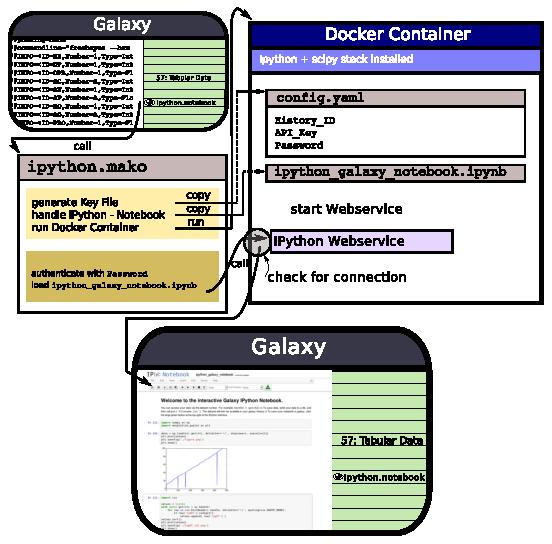
\includegraphics{diagram.pdf}}
\caption{Diagram of the program flow when the IPython Visualization is used. The IPython visualization plugin is divided into two parts, the first part generates a key file and generates an IPython notebook, then it runs a container from a specific Docker image. In this Docker container, IPython and all its dependencies are installed as well as some Python libraries. The key file and the IPython notebook are copied to the container and the IPython Webservice is started. The second part of the visualization template now generates a connection to the web service provided by the Docker container. For clean keeping the container also checks whether or not a connection to it exists. If the container is no longer used it terminates itself.}
\label{fig:diagram}
\end{figure}


\end{methods}


%%%%%%%%%%%%%%%%%%%%%%%%%%%%%%%%%%%%%%%%%%%%%%%%%%%%%%%%%%%%%%%%%%%%%%%%%%%%%%%%%%%%%
%
%     please remove the " % " symbol from \centerline{\includegraphics{fig01.eps}}
%     as it may ignore the figures.
%
%%%%%%%%%%%%%%%%%%%%%%%%%%%%%%%%%%%%%%%%%%%%%%%%%%%%%%%%%%%%%%%%%%%%%%%%%%%%%%%%%%%%%%


\section{Conclusion}
The IPython-Docker container adds versatility to Galaxy by embedding a Python shell in a secure and easy to install manner. This plugin represents a major shortcut for anybody with some programming experience who can not wait for a specific tool to be implemented in Galaxy or who needs more control to manipulate data. The possibilities with this plugin are immense and the small example is just a glimpse of what could be done with a fully implemented scipy stack. The major security concern of giving a user access to such a powerful tool such as IPython has been taken care of by putting the IPython web service inside a Docker container. This puts the user in a sandbox and isolates him from the rest of the system such that he can not break the system or read sensitive data from other users. The user can interact with the Galaxy instance with the two predefined functions \textit{put} and \textit{get} and these two functions essentially define the exchange between the container and the Galaxy instance. With the possibility to store the IPython notebook in the history, consistent and reproducible data analysis is possible and encouraged. By publishing or sharing a history containing IPython notebooks, notebooks can be easily shared with other users. That way users with no programming experience can benefit from notebooks developed by users with programming experience. 



\section*{Acknowledgement}
We would like to thank the Galaxy team and the Galaxy community for being so inspiring and helpful. 


\paragraph{Funding\textcolon} The project was supported by the German Research Foundation (DFG-grant SFB 992/1).

\bibliographystyle{natbib}
%\bibliographystyle{achemnat}
%\bibliographystyle{plainnat}
%\bibliographystyle{abbrv}
%\bibliographystyle{bioinformatics}
%
%\bibliographystyle{plain}
%
%\bibliography{Document}


\begin{thebibliography}{}
\bibitem[Blankenberg {\it et~al}., 2010]{Blank2010}
Blankenberg, A. {\it et~al}., (2010) Galaxy: a web-based genome analysis tool for experimentalists. \textit{Curr. Protoc. Mol. Biol.},  {\bf Chapter 19}, Unit 19.10.1-21.

\bibitem[Giardine {\it et~al}., 2005]{Giardine2005}
Giardine, D. {\it et~al}., (2005) Galaxy: a platform for interactive large-scale genome analysis. \textit{Genome Res.},  {\bf 15}, 1451-1455.

\bibitem[Goecks {\it et~al}., 2010]{Goecks2010}
Goecks, J. {\it et~al}., (2005) Galaxy: a comprehensive approach for supporting accessible, reproducible, and transparent computational research in the life sciences. \textit{Genome Biol.},  {\bf 11}, R86.

\bibitem[P\'erez {\it et~al}., 2007]{Perez2007}
P\'erez, F. {\it et~al}., (2007) IPython: A System for Interactive Scientific Computing. \textit{Comput. Sci. Eng.}, {\bf 9}, 21-29.

\bibitem[Sloggett {\it et~al}., 2013]{Sloggett2013}
Sloggett, C. {\it et~al}., (2013) BioBlend: automating pipeline analyses within Galaxy and CloudMan. \textit{Bioinformatics}, {\bf 29}, 1685-1686.

\bibitem[Blankenberg {\it et~al}., 2014]{Blankenberg2014}
Blankenberg, A. {\it et~al}., (2014) Dissemination of scientific software with Galaxy ToolShed. \textit{Genome Biol.}, {\bf 15}, 403.



\end{thebibliography}
\end{document}
